\chapter{द्विपरमाणुक अणुओं के आण्विक कक्षक}\label{ch:b2:diatomic-mos}

किसी प्रबल चुंबक के ध्रुवों के बीच द्रव ऑक्सीजन उँडेलिए, वह एक ओर खिंच
जाती है; द्रव नाइट्रोजन सीधे नीचे गिरती है। ऑक्सीजन अणु में
अयुग्मित इलेक्ट्रॉन होते हैं, जिन्हें चुंबकीय क्षेत्र आकर्षित करता है। उसकी लुइस संरचना,
\ce{O=O}, जिसमें हर इलेक्ट्रॉन युग्मित है, यह नहीं बता सकती। \omterm{def:b2:diatomic-mos:lcao}{आण्विक कक्षक},
जो पिछले अध्याय के परमाण्वीय कक्षकों से बनते हैं, किसी अणु के हर इलेक्ट्रॉन को
उसके अपने स्तर में रखते हैं: वे ऑक्सीजन के चुंबकत्व, आबंधों की प्रबलता और
लंबाई, और अणुओं को आयनित करने के लिए आवश्यक ऊर्जाओं की व्याख्या करते हैं --- और
आगे के अध्यायों की अभिक्रियाशीलता की नींव रखते हैं।

\begin{recall}
\Cref{ch:b2:atomic-orbitals}: परमाण्वीय कक्षक, उनकी आकृतियाँ, चिह्न और
ऊर्जाएँ। प्रथम वर्ष का खंड: लुइस संरचनाएँ, वर्णनात्मक धारणाओं के रूप में $\sigma$ और $\pi$
आबंध, संकरण और उसकी सीमाएँ, अयुग्मित इलेक्ट्रॉन और
मूलक।
\end{recall}

\begin{omfigure}
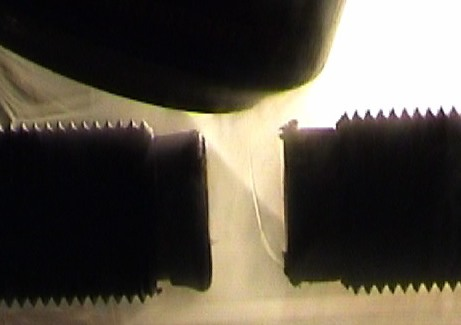
\includegraphics[width=0.42\linewidth]{images/book3/liquid-oxygen.jpg}

{\small द्रव ऑक्सीजन की एक पतली धारा, जो किसी प्रबल चुंबक के ध्रुवों के बीच
गिरती है, उनकी ओर खिंचती है और एक सेतु की तरह लटक जाती है: अणु
\omterm{def:b2:diatomic-mos:magnetism}{अनुचुंबकीय} है। (छायाचित्र: पीटर काउपर, सार्वजनिक अधिकार-क्षेत्र, विकिमीडिया कॉमन्स।)}
\end{omfigure}

\section{LCAO विधि}

\begin{definition}[आण्विक कक्षक]\label{def:b2:diatomic-mos:lcao}
\emph{आण्विक कक्षक}\index{आण्विक कक्षक} किसी अणु में एक
इलेक्ट्रॉन का \omterm{def:b2:atomic-orbitals:wavefunction}{तरंग फलन} है, जो उसके सभी नाभिकों पर फैला होता है। \emph{LCAO}\index{LCAO}
विधि (परमाण्वीय कक्षकों का रैखिक संयोजन) में इसे परमाणुओं के परमाण्वीय
कक्षकों के योग, $\psi = \sum_i c_i\varphi_i$, के रूप में लिखा जाता है, जिसके गुणांक
ऊर्जा को न्यूनतम करने के लिए चुने जाते हैं।
\end{definition}

दो परमाणुओं A और B के लिए, जो एक-एक कक्षक लाते हैं, $\psi = c_A\varphi_A + c_B\varphi_B$।
$\psi$ में इलेक्ट्रॉन की ऊर्जा, गुणांकों के सापेक्ष न्यूनतमीकृत करने पर,
तीन संख्याएँ सामने लाती है।

\begin{definition}[LCAO विधि के समाकल]\label{def:b2:diatomic-mos:integrals}
दो वास्तविक परमाण्वीय कक्षकों $\varphi_A$, $\varphi_B$ और अणु में किसी इलेक्ट्रॉन के
ऊर्जा संकारक $\hat H$ के लिए:
\begin{itemize}
  \item \emph{अतिव्यापन समाकल}\index{अतिव्यापन समाकल} $S = \int\varphi_A\varphi_B\,dV$
        मापता है कि दोनों कक्षक कितना एक ही क्षेत्र घेरते हैं (सर्वसम,
        अध्यारोपित कक्षकों के लिए $S = 1$);
  \item \emph{कूलॉम समाकल}\index{कूलॉम समाकल} $\alpha_A = \int\varphi_A\hat
        H\varphi_A\,dV$ अणु के भीतर $\varphi_A$ में इलेक्ट्रॉन की ऊर्जा है,
        परमाण्वीय \omterm{def:b2:atomic-orbitals:orbital-energy}{कक्षक ऊर्जा} के निकट;
  \item \emph{अनुनाद समाकल}\index{अनुनाद समाकल} $\beta = \int\varphi_A\hat
        H\varphi_B\,dV$, ऋणात्मक, दोनों कक्षकों के युग्मन को मापता है।
\end{itemize}
\omterm{def:b2:diatomic-mos:lcao}{आण्विक कक्षकों} की ऊर्जाएँ $E$ इस \emph{सेकुलर
सारणिक}\index{सेकुलर सारणिक} के मूल हैं:
\[
  \begin{vmatrix} \alpha_A - E & \beta - ES \\ \beta - ES & \alpha_B - E \end{vmatrix} = 0 .
\]
\end{definition}

सारणिक $E = \int\psi\hat H\psi\,dV/\int\psi^2\,dV$ को $c_A$ और $c_B$ के सापेक्ष
न्यूनतम करने से आता है: दोनों शर्तें $\partial E/\partial c_A =
\partial E/\partial c_B = 0$ एक समघात रैखिक निकाय बनाती हैं, जिसका शून्येतर
हल तभी होता है जब उसका सारणिक शून्य हो। वह विचरण चरण यहाँ स्वीकार
किया गया है।

\begin{theorem}[दो सर्वसम कक्षक]\label{thm:b2:diatomic-mos:homonuclear}
$\alpha_A = \alpha_B = \alpha$ के लिए दोनों \omterm{def:b2:diatomic-mos:lcao}{आण्विक कक्षक} ये हैं:
\[
  E_+ = \frac{\alpha + \beta}{1 + S}, \quad \psi_+ = \frac{\varphi_A + \varphi_B}{\sqrt{2(1 + S)}} ;
  \qquad
  E_- = \frac{\alpha - \beta}{1 - S}, \quad \psi_- = \frac{\varphi_A - \varphi_B}{\sqrt{2(1 - S)}} .
\]
\end{theorem}

\begin{proof}
सारणिक $(\alpha - E)^2 = (\beta - ES)^2$ देता है, अतः $\alpha - E = \pm(\beta - ES)$।
धन चिह्न के साथ $E(1 + S) = \alpha + \beta$; ऋण चिह्न के साथ $E(1 - S) = \alpha
- \beta$। रैखिक निकाय में वापस रखने पर $(\alpha - E)c_A + (\beta - ES)c_B = 0$ से $c_B
= c_A$ मिलता है $E_+$ के लिए, और $c_B = -c_A$ मिलता है $E_-$ के लिए। प्रसामान्यीकरण: $\int(\varphi_A \pm
\varphi_B)^2\,dV = 2 \pm 2S$।
\end{proof}

\begin{definition}[आबंधी और प्रतिआबंधी कक्षक]\label{def:b2:diatomic-mos:bonding}
\emph{आबंधी कक्षक}\index{आबंधी कक्षक} उन परमाण्वीय कक्षकों से नीचे होता है जिनसे वह
बना है: उसका इलेक्ट्रॉन घनत्व नाभिकों के बीच संचित होता है।
\emph{प्रतिआबंधी कक्षक}\index{प्रतिआबंधी कक्षक} उनसे ऊपर होता है और नाभिकों के बीच
उसका एक नोडीय तल होता है। \emph{अनाबंधी कक्षक}\index{अनाबंधी कक्षक}
परमाण्वीय कक्षक की ऊर्जा बनाए रखता है, जिसे संयोजित होने के लिए कोई
साथी नहीं मिलता।
\end{definition}

\begin{proposition}[प्रतिआबंधी कक्षक अधिक ऊपर उठता है]\label{prop:b2:diatomic-mos:asymmetry}
$S > 0$ के लिए प्रतिआबंधी स्तर $\alpha$ से जितना ऊपर उठता है, आबंधी स्तर
उससे उतना नीचे नहीं जाता, कम जाता है।
\end{proposition}

\begin{proof}
$E_+ - \alpha = (\beta - \alpha S)/(1 + S)$ और $E_- - \alpha = -(\beta - \alpha S)/(1 - S)$।
अंश $\beta - \alpha S$ ऋणात्मक है (युग्मन प्रभावी है), और $1 - S < 1
+ S$: दूसरा विस्थापन परिमाण में बड़ा है।
\end{proof}

दो इलेक्ट्रॉनों के साथ, जैसे \ce{H2} में, दोनों $\psi_+$ में जाते हैं और अणु
अलग परमाणुओं से अधिक स्थायी है। चार के साथ, जैसे \ce{He2} में, दो को $\psi_-$ में जाना पड़ता है,
जिसकी लागत $\psi_+$ के लाभ से अधिक है: \ce{He2} बद्ध नहीं है।

\begin{omfigure}
\begin{MOdiagram}[names, labels]
  \atom[H]{left}{ 1s = {0;up} }
  \atom[H]{right}{ 1s = {0;up} }
  \molecule[\ce{H2}]{ 1sMO = {.75;pair} }
\end{MOdiagram}
\hspace{1.5cm}
\begin{MOdiagram}[names, labels]
  \atom[He]{left}{ 1s = {0;pair} }
  \atom[He]{right}{ 1s = {0;pair} }
  \molecule[\ce{He2}]{ 1sMO = {.75;pair,pair} }
\end{MOdiagram}

{\small \ce{H2} (\omterm{def:b2:diatomic-mos:bond-order}{आबंध कोटि} 1) और \ce{He2} (\omterm{def:b2:diatomic-mos:bond-order}{आबंध
कोटि} 0, बद्ध नहीं) के \omterm{def:b2:diatomic-mos:lcao}{आण्विक कक्षक} आरेख। हर खाना एक स्तर है जिसमें विपरीत चक्रणों वाले अधिकतम
दो इलेक्ट्रॉन होते हैं; खंडित रेखाएँ हर \omterm{def:b2:diatomic-mos:lcao}{आण्विक कक्षक} को उन परमाण्वीय कक्षकों से जोड़ती हैं
जिनसे वह बना है।}
\end{omfigure}

\section{अतिव्यापन और सममिति}

\begin{definition}[$\sigma$ और $\pi$ कक्षक]\label{def:b2:diatomic-mos:sigma-pi}
किसी रैखिक अणु का \emph{$\sigma$ कक्षक}\index{सिग्मा कक्षक@$\sigma$ कक्षक} आण्विक अक्ष के परितः किसी भी
घूर्णन से अपरिवर्तित रहता है: उसका कोई नोडीय तल अक्ष को समाविष्ट नहीं करता।
\emph{$\pi$ कक्षक}\index{पाई कक्षक@$\pi$ कक्षक} अक्ष के परितः $180^\circ$ के घूर्णन में चिह्न बदलता है:
उसका एक नोडीय तल अक्ष को समाविष्ट करता है। तारांक \omterm{def:b2:diatomic-mos:bonding}{प्रतिआबंधी
कक्षकों} को चिह्नित करता है ($\sigma^*$, $\pi^*$)।
\end{definition}

\begin{proposition}[सममिति से शून्य अतिव्यापन]\label{prop:b2:diatomic-mos:symmetry}
ऐसे दो कक्षक, जिनमें से एक आण्विक अक्ष को समाविष्ट करने वाले किसी तल के सापेक्ष सममित और
दूसरा प्रतिसममित है, शून्य अतिव्यापन और शून्य \omterm{def:b2:diatomic-mos:integrals}{अनुनाद
समाकल} रखते हैं: वे संयोजित नहीं होते।
\end{proposition}

\begin{proof}
तल में परावर्तन आकाश को अपरिवर्तित छोड़ता है, परंतु गुणनफल
$\varphi_A\varphi_B$ को दर्पण-बिंदु पर उसके विपरीत में बदल देता है: $\int\varphi_A\varphi_B\,dV$ में
आकाश के दोनों अर्धों के योगदान कट जाते हैं। यही
$\int\varphi_A\hat H\varphi_B\,dV$ के लिए भी सत्य है, क्योंकि $\hat H$ में अणु की सममिति है।
\end{proof}

दो कक्षक तब प्रबल अन्योन्यक्रिया करते हैं जब उनकी सममिति समान हो (शून्येतर
अतिव्यापन), वे अच्छी तरह अतिव्यापित हों, और निकट ऊर्जाओं पर हों। एक परमाणु का 1s कक्षक और
दूसरे का $2\mathrm p_x$ ($x$ अक्ष के लंबवत) कभी संयोजित नहीं होते;
$2\mathrm p_z$ कक्षक (अक्ष के अनुदिश) $\sigma$ कक्षक देते हैं; $2\mathrm p_x$ और
$2\mathrm p_y$ समान ऊर्जाओं वाले $\pi$ कक्षकों के दो युग्म देते हैं।

\begin{omfigure}
\begin{tikzpicture}[font=\small]
  % sigma 1s
  \pic at (0,0) {oms={0.85}}; \pic at (0.7,0) {oms={0.85}};
  \node at (0.35,-0.75) {$\sigma_{1s}$};
  \pic at (2.2,0) {oms={0.85}}; \pic at (2.9,0) {oms={-0.85}};
  \node at (2.55,-0.75) {$\sigma^*_{1s}$};
  % sigma 2p
  \pic at (4.6,0) {omp={-1}{0}}; \pic at (5.6,0) {omp={1}{0}};
  \node at (5.1,-0.75) {$\sigma_{2p}$};
  \pic at (7.4,0) {omp={-1}{0}}; \pic at (8.6,0) {omp={-1}{0}};
  \node at (8.0,-0.75) {$\sigma^*_{2p}$};
  % pi 2p
  \pic at (10.2,0) {omp={1}{90}}; \pic at (10.9,0) {omp={1}{90}};
  \node at (10.55,-0.95) {$\pi_{2p}$};
  \pic at (12.2,0) {omp={1}{90}}; \pic at (12.9,0) {omp={-1}{90}};
  \node at (12.55,-0.95) {$\pi^*_{2p}$};
  \draw[black!40, dashed] (-0.6,0) -- (13.4,0);
\end{tikzpicture}

{\small किसी समनाभिकीय द्विपरमाणुक के \omterm{def:b2:diatomic-mos:lcao}{आण्विक कक्षक}, व्यवस्था-रूप (आण्विक
अक्ष क्षैतिज और खंडित है)। समकला संयोजन (आबंधी) नाभिकों के बीच
एक ही रंग इकट्ठा करते हैं; विषमकला संयोजन (प्रतिआबंधी) उनके बीच एक
नोडीय तल रखते हैं। $\sigma$ कक्षक अक्ष के परितः सममित हैं; हर $\pi$
कक्षक का नोडीय तल अक्ष को समाविष्ट करता है।}
\end{omfigure}

\section{आवर्त 2 के समनाभिकीय द्विपरमाणुक}

आवर्त 2 के दो परमाणुओं के 2s और 2p कक्षकों से आठ \omterm{def:b2:diatomic-mos:lcao}{आण्विक कक्षक}
बनते हैं: $\sigma_{2s}$, $\sigma^*_{2s}$, $\sigma_{2p}$, दो $\pi_{2p}$, दो $\pi^*_{2p}$,
$\sigma^*_{2p}$।

\begin{proposition}[s और p का मिश्रण]\label{prop:b2:diatomic-mos:sp-mixing}
\ce{O2} और \ce{F2} के लिए क्रम $\sigma_{2s} < \sigma^*_{2s} < \sigma_{2p} < \pi_{2p} <
\pi^*_{2p} < \sigma^*_{2p}$ है। \ce{Li2} से \ce{N2} तक, जिनके 2s और 2p स्तर निकट हैं,
वे $\sigma$ कक्षक, जो 2s और $2\mathrm p_z$ से बने हैं, मिश्रित होते हैं: $\sigma_{2p}$ ऊपर धकेलकर
$\pi_{2p}$ से ऊपर पहुँच जाता है।
\end{proposition}

\begin{proof}[तर्क]
$\sigma_{2s}$ और $\sigma_{2p}$ कक्षकों की सममिति समान है और वे एक-दूसरे से
संयोजित हो सकते हैं। समान सममिति के दो स्तर एक-दूसरे को प्रतिकर्षित करते हैं (नीचे
\cref{thm:b2:diatomic-mos:heteronuclear}): $\sigma_{2s}$ नीचे जाता है, $\sigma_{2p}$ ऊपर, और जितने
वे निकट हों उतना अधिक। आवर्त के अनुदिश 2s--2p अंतराल बढ़ता है, इसलिए प्रभाव बाईं ओर बड़ा
और ऑक्सीजन तथा फ़्लुओरीन के लिए छोटा है। नाइट्रोजन और ऑक्सीजन के बीच का संक्रमण
मापे गए प्रकाशइलेक्ट्रॉन स्पेक्ट्रमों से स्वीकार किया गया है।
\end{proof}

\begin{definition}[आबंध कोटि]\label{def:b2:diatomic-mos:bond-order}
किसी द्विपरमाणुक अणु की \emph{आबंध कोटि}\index{आबंध कोटि} $b = (n_b -
n_a)/2$ है, जहाँ $n_b$ और $n_a$ आबंधी और \omterm{def:b2:diatomic-mos:bonding}{प्रतिआबंधी कक्षकों} में इलेक्ट्रॉनों की
संख्याएँ हैं।
\end{definition}

\begin{proposition}[आबंध कोटि और आबंध]\label{prop:b2:diatomic-mos:bond-order}
तत्वों के एक ही युग्म के परमाणुओं के बीच ऊँची \omterm{def:b2:diatomic-mos:bond-order}{आबंध कोटि}
छोटे और प्रबलतर आबंध के साथ आती है; शून्य \omterm{def:b2:diatomic-mos:bond-order}{आबंध कोटि} का अर्थ है कोई आबंध नहीं।
\end{proposition}

\begin{proof}[तर्क]
हर आबंधी इलेक्ट्रॉन नाभिकों के बीच घनत्व जोड़ता है और ऊर्जा घटाता है;
हर प्रतिआबंधी इलेक्ट्रॉन उसे हटाता है और ऊर्जा को कम से कम उतना ही बढ़ाता है
(\cref{prop:b2:diatomic-mos:asymmetry})। आबंधी युग्मों की शुद्ध संख्या
बंधन को मापती है। तुलना केवल समान परमाणुओं के लिए अर्थपूर्ण है: \ce{Li2} की
\omterm{def:b2:diatomic-mos:bond-order}{आबंध कोटि} \ce{F2} की तरह 1 है, परंतु उसके 2s कक्षक कहीं बड़े हैं।
\end{proof}

\begin{definition}[अनुचुंबकीय और प्रतिचुंबकीय]\label{def:b2:diatomic-mos:magnetism}
कोई पदार्थ \emph{अनुचुंबकीय}\index{अनुचुंबकीय} है यदि उसके अणुओं में
अयुग्मित इलेक्ट्रॉन हों: वह चुंबकीय क्षेत्र में खिंचता है। वह
\emph{प्रतिचुंबकीय}\index{प्रतिचुंबकीय} है यदि उसके सभी इलेक्ट्रॉन युग्मित हों: वह
क्षेत्र से दुर्बलता से बाहर धकेला जाता है।
\end{definition}

\begin{omfigure}
\begin{MOdiagram}[names, labels, style=square, distance=4.2cm, labels-fs=\scriptsize]
  \atom[N]{left}{ 2s = {0;pair}, 2p = {3.5;up,up,up} }
  \atom[N]{right}{ 2s = {0;pair}, 2p = {3.5;up,up,up} }
  \molecule[\ce{N2}]{ 2sMO = {.7;pair,pair}, 2pMO = {0.4/2.5,1.4;pair,pair,pair} }
\end{MOdiagram}
\hfill
\begin{MOdiagram}[names, labels, style=square, distance=4.2cm, labels-fs=\scriptsize]
  \atom[O]{left}{ 2s = {0;pair}, 2p = {3.5;pair,up,up} }
  \atom[O]{right}{ 2s = {0;pair}, 2p = {3.5;pair,up,up} }
  \molecule[\ce{O2}]{ 2sMO = {.7;pair,pair}, 2pMO = {1.8,.8;pair,pair,pair,up,up} }
\end{MOdiagram}

{\small \ce{N2} (बाएँ, s और p का मिश्रण के साथ:
$\sigma_{2p}$, $\pi_{2p}$ से ऊपर) और \ce{O2} (दाएँ) के संयोजकता \omterm{def:b2:diatomic-mos:lcao}{आण्विक कक्षक} आरेख। नाइट्रोजन: \omterm{def:b2:diatomic-mos:bond-order}{आबंध कोटि}
$(8 - 2)/2 = 3$, सभी इलेक्ट्रॉन युग्मित। ऑक्सीजन: \omterm{def:b2:diatomic-mos:bond-order}{आबंध कोटि} $(8 - 4)/2 = 2$, दो
$\pi^*$ कक्षकों में दो अयुग्मित इलेक्ट्रॉनों के साथ (हुंड का नियम): \ce{O2}
\omterm{def:b2:diatomic-mos:magnetism}{अनुचुंबकीय} है। आरेख $x$ को आण्विक अक्ष लेते हैं, इसीलिए नाम
$2\sigma_x$, $2\pi_y$, $2\pi_z$ हैं।}
\end{omfigure}

\begin{method}[आण्विक कक्षक आरेख बनाना और भरना]\label{met:b2:diatomic-mos:build-diagram}
\begin{enumerate}
  \item हर परमाणु के संयोजकता परमाण्वीय कक्षकों को उनकी ऊर्जाओं पर रखिए, अधिक
        विद्युत-ऋणात्मक परमाणु को नीचे।
  \item समान सममिति के कक्षकों को संयोजित कीजिए: हर युग्म नीचे एक \omterm{def:b2:diatomic-mos:bonding}{आबंधी कक्षक}
        और ऊपर एक \omterm{def:b2:diatomic-mos:bonding}{प्रतिआबंधी कक्षक} देता है; बिना साथी का कक्षक
        अनाबंधी रहता है।
  \item आवर्त 2 के समनाभिकीय अणुओं के लिए नाइट्रोजन तक $\sigma_{2p}$ को
        $\pi_{2p}$ से ऊपर, और ऑक्सीजन से आगे उससे नीचे वाला क्रम प्रयुक्त कीजिए।
\end{enumerate}
\end{method}

\begin{method}[भरे हुए आरेख को पढ़ना]\label{met:b2:diatomic-mos:fill}
\begin{enumerate}
  \item संयोजकता इलेक्ट्रॉन गिनिए (हर ऋणात्मक आवेश के लिए एक जोड़िए, हर
        धनात्मक आवेश के लिए एक घटाइए)।
  \item नीचे से भरिए, प्रति कक्षक दो, अपभ्रष्ट स्तरों के लिए हुंड के नियम के
        साथ।
  \item \omterm{def:b2:diatomic-mos:bond-order}{आबंध कोटि} $(n_b - n_a)/2$; अयुग्मित इलेक्ट्रॉन अनुचुंबकत्व देते हैं।
  \item उच्चतम भरा स्तर वह है जो पहले आयनित होता है।
\end{enumerate}
\end{method}

\begin{omfigure}
\small
\renewcommand{\arraystretch}{1.15}
\begin{tabular}{lcccccc}
 & \ce{Li2} & \ce{C2} & \ce{N2} & \ce{O2} & \ce{F2} & \ce{NO} \\ \hline
संयोजकता इलेक्ट्रॉन & 2 & 8 & 10 & 12 & 14 & 11 \\
\omterm{def:b2:diatomic-mos:bond-order}{आबंध कोटि} & 1 & 2 & 3 & 2 & 1 & 2.5 \\
अयुग्मित इलेक्ट्रॉन & 0 & 0 & 0 & 2 & 0 & 1 \\
आबंध लंबाई $r_e$ (pm) & 267.3 & 124.3 & 109.8 & 120.8 & 141.2 & 115.1 \\
$D_0$ (\unit{eV}) & 1.04 & 6.15 & 9.76 & 5.12 & 1.60 & 6.51 \\
\end{tabular}

\smallskip
{\small आवर्त-2 के द्विपरमाणुक: \omterm{def:b2:diatomic-mos:lcao}{आण्विक कक्षक} आरेखों से \omterm{def:b2:diatomic-mos:bond-order}{आबंध कोटियाँ}; आबंध लंबाइयाँ
स्पेक्ट्रमिकी से, वियोजन ऊर्जाएँ $D_0$ \qty{0}{K} पर सारणीबद्ध संभवन एन्थैल्पियों से,
$D_0 = \Delta_f H_0(\mathrm A) + \Delta_f H_0(\mathrm B) - \Delta_f
H_0(\mathrm{AB})$।}
% ledger: re:Li2, re:C2, re:N2, re:O2, re:F2, re:NO, janafH0:Li, janafH0:Li2, janafH0:C, janafH0:C2, janafH0:N, janafH0:O, janafH0:F, janafH0:NO
\end{omfigure}

\section{विषमनाभिकीय द्विपरमाणुक}

\begin{theorem}[भिन्न ऊर्जाओं वाले दो कक्षक]\label{thm:b2:diatomic-mos:heteronuclear}
$\alpha_A > \alpha_B$ (B अधिक विद्युत-ऋणात्मक) के लिए, $S$ नगण्य मानकर, $\bar\alpha = (\alpha_A
+ \alpha_B)/2$ और $\Delta = \alpha_A - \alpha_B$ के साथ:
\[
  E_\mp = \bar\alpha \mp \sqrt{\Delta^2/4 + \beta^2} .
\]
\omterm{def:b2:diatomic-mos:bonding}{आबंधी कक्षक} (नीचा) का बड़ा गुणांक B पर होता है, \omterm{def:b2:diatomic-mos:bonding}{प्रतिआबंधी
कक्षक} का A पर; जब $\Delta \gg |\beta|$, तो $E_- \approx \alpha_B - \beta^2/\Delta$ और $E_+
\approx \alpha_A + \beta^2/\Delta$।
\end{theorem}

\begin{proof}
$S = 0$ के साथ ऊर्जाएँ $\begin{pmatrix}\alpha_A & \beta \\
\beta & \alpha_B\end{pmatrix}$ के अभिलक्षणिक मान हैं: $(\alpha_A - E)(\alpha_B - E) = \beta^2$, जिसके मूल
$\bar\alpha \pm \sqrt{\Delta^2/4 + \beta^2}$ हैं। निचले मूल के लिए $(\alpha_B - E_-)c_B = -\beta
c_A$; $\alpha_B - E_- = \sqrt{\Delta^2/4 + \beta^2} - \Delta/2$, $|\beta|$ से छोटा है, अतः
$|c_A| < |c_B|$। $\Delta \gg |\beta|$ के लिए $\sqrt{\Delta^2/4 + \beta^2} \approx \Delta/2 +
\beta^2/\Delta$।
\end{proof}

\begin{omfigure}
\begin{tikzpicture}
\begin{axis}[width=0.55\linewidth, height=6cm, xmin=0, xmax=8, ymin=-5, ymax=5,
  axis x line=bottom, axis y line=left, xlabel={$\Delta/|\beta|$}, ylabel={$E/|\beta|$},
  tick label style={font=\small}, label style={font=\small}]
\addplot[omThm, thick] table[x=d, y=Ehigh] {figdata/out/bachelor-2-two-level-a.dat};
\addplot[omDef, thick] table[x=d, y=Elow] {figdata/out/bachelor-2-two-level-a.dat};
\addplot[black!50, densely dotted] table[x=d, y=aA] {figdata/out/bachelor-2-two-level-a.dat};
\addplot[black!50, densely dotted] table[x=d, y=aB] {figdata/out/bachelor-2-two-level-a.dat};
\addplot[omThm, dashed] table[x=d, y=Phigh] {figdata/out/bachelor-2-two-level-a-pert.dat};
\addplot[omDef, dashed] table[x=d, y=Plow] {figdata/out/bachelor-2-two-level-a-pert.dat};
\node[font=\scriptsize, black!60, anchor=north west] at (axis cs:5.5,2.6) {$\alpha_A$};
\node[font=\scriptsize, black!60, anchor=south west] at (axis cs:5.5,-2.6) {$\alpha_B$};
\node[font=\scriptsize, omThm, anchor=south east] at (axis cs:3.2,2.2) {प्रतिआबंधी};
\node[font=\scriptsize, omDef, anchor=north east] at (axis cs:3.2,-2.2) {आबंधी};
\end{axis}
\end{tikzpicture}

{\small दो अन्योन्यक्रियारत स्तर। परमाण्वीय कक्षकों के बीच अंतराल $\Delta$ बढ़ने पर
आण्विक स्तर (ठोस रेखाएँ) परमाण्वीय स्तरों (बिंदुकित) के निकट आते हैं: विक्षोभ
सीमा (खंडित) का स्थायीकरण $\beta^2/\Delta$ छोटा हो जाता है। $\Delta = 0$ पर
विपाटन $2|\beta|$ है।}
\end{omfigure}

हाइड्रोजन फ़्लुओराइड में हाइड्रोजन का 1s कक्षक फ़्लुओरीन के कहीं नीचे के 2p कक्षकों से
मिलता है। केवल अक्ष के अनुदिश $2\mathrm p_z$ की सममिति सही है: यह
फ़्लुओरीन पर भारित एक $\sigma$ \omterm{def:b2:diatomic-mos:bonding}{आबंधी कक्षक}, और हाइड्रोजन पर भारित एक $\sigma^*$
बनाता है। फ़्लुओरीन के $2\mathrm p_x$ और $2\mathrm p_y$ कक्षक
अनाबंधी रहते हैं: वे उसके एकाकी युग्म हैं। आबंध फ़्लुओरीन की ओर ध्रुवित है।

कार्बन मोनॉक्साइड में \ce{N2} के दस संयोजकता इलेक्ट्रॉन और मिलता-जुलता आरेख है,
परंतु ऑक्सीजन के कक्षक नीचे हैं। इसके \omterm{def:b2:diatomic-mos:bonding}{आबंधी कक्षक} ऑक्सीजन पर भारित हैं;
इसका उच्चतम भरा कक्षक, कार्बन पर भारित एक $\sigma$ कक्षक, कार्बन पर एक एकाकी युग्म
है। इसलिए कार्बन मोनॉक्साइड धातुओं से कार्बन के माध्यम से बंधित होती है
(\cref{ch:b2:coordination-complexes})।

\begin{omfigure}
\begin{tikzpicture}[font=\small]
  % CO schematic: C left (higher), O right (lower)
  \pic (c2s) at (0,0.6) {omlevel={ud}{0.8}}; \node[left] at (-0.5,0.6) {2s};
  \pic (c2p1) at (-0.45,2.6) {omlevel={u}{0.4}}; \pic (c2p2) at (0,2.6) {omlevel={u}{0.4}}; \pic (c2p3) at (0.45,2.6) {omlevel={empty}{0.4}};
  \node[left] at (-0.75,2.6) {2p};
  \node at (0,-0.6) {C};
  \pic (o2s) at (6,-1.2) {omlevel={ud}{0.8}}; \node[right] at (6.5,-1.2) {2s};
  \pic (o2p1) at (5.55,1.4) {omlevel={ud}{0.4}}; \pic (o2p2) at (6,1.4) {omlevel={u}{0.4}}; \pic (o2p3) at (6.45,1.4) {omlevel={u}{0.4}};
  \node[right] at (6.75,1.4) {2p};
  \node at (6,-2.2) {O};
  % MOs
  \pic (m1) at (3,-1.8) {omlevel={ud}{0.8}};
  \pic (m2) at (3,-0.2) {omlevel={ud}{0.8}};
  \pic (m3a) at (2.75,0.9) {omlevel={ud}{0.45}}; \pic (m3b) at (3.25,0.9) {omlevel={ud}{0.45}};
  \pic (m4) at (3,1.9) {omlevel={ud}{0.8}};
  \pic (m5a) at (2.75,3.3) {omlevel={empty}{0.45}}; \pic (m5b) at (3.25,3.3) {omlevel={empty}{0.45}};
  \pic (m6) at (3,4.4) {omlevel={empty}{0.8}};
  \draw[omcorr, densely dashed] (c2s-r) -- (m1-l) (o2s-l) -- (m1-r);
  \draw[omcorr, densely dashed] (c2s-r) -- (m2-l) (o2s-l) -- (m2-r);
  \draw[omcorr, densely dashed] (c2p3-r) -- (m3a-l) (o2p1-l) -- (m3b-r);
  \draw[omcorr, densely dashed] (c2p3-r) -- (m4-l) (o2p1-l) -- (m4-r);
  \draw[omcorr, densely dashed] (c2p3-r) -- (m5a-l) (o2p1-l) -- (m5b-r);
  \draw[omcorr, densely dashed] (c2p3-r) -- (m6-l) (o2p1-l) -- (m6-r);
  \node[omsymlabel, below=0.17cm, inner sep=0.5pt] at (m1-c) {$\sigma$};
  \node[omsymlabel, below=0.17cm, inner sep=0.5pt] at (m2-c) {$\sigma$};
  \node[omsymlabel, below=0.17cm, inner sep=0.5pt] at (3,0.9) {$\pi$};
  \node[omsymlabel, below=0.24cm, inner sep=0.5pt] at (m4-c) {$\sigma$ (C का एकाकी युग्म)};
  \node[omsymlabel, below=0.05cm, inner sep=0.5pt] at (3,3.3) {$\pi^*$};
  \node[omsymlabel, below=0.05cm, inner sep=0.5pt] at (m6-c) {$\sigma^*$};
  \node at (3,-2.6) {CO};
\end{tikzpicture}

{\small कार्बन मोनॉक्साइड के संयोजकता कक्षक, व्यवस्था-रूप: ऑक्सीजन के कक्षक कार्बन के
कक्षकों से नीचे हैं। \ce{N2} की तरह \omterm{def:b2:diatomic-mos:bond-order}{आबंध कोटि} 3; उच्चतम भरा
कक्षक कार्बन पर भारित एक $\sigma$ कक्षक है, उसका एकाकी युग्म।}
\end{omfigure}

\begin{history}[हुंड और मुलिकेन]
\begin{minipage}[t]{0.27\linewidth}
\vspace{0pt}
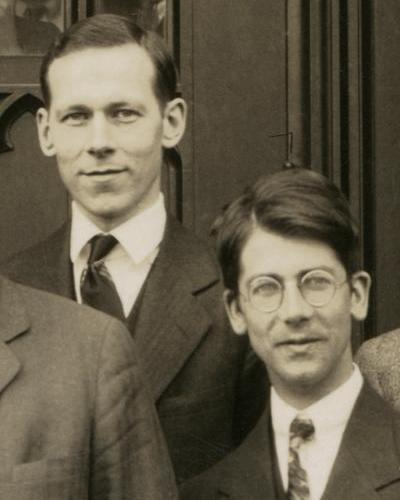
\includegraphics[width=\linewidth]{images/book3/mulliken-hund.jpg}
\end{minipage}\hfill
\begin{minipage}[t]{0.69\linewidth}
\vspace{0pt}
1926 और 1932 के बीच फ़्रीडरिख हुंड और रॉबर्ट मुलिकेन ने द्विपरमाणुक अणुओं के
स्पेक्ट्रमों की व्याख्या हर इलेक्ट्रॉन को पूरे अणु के एक कक्षक से संबद्ध करके की,
जिसे अक्ष के परितः उसकी सममिति से वर्गीकृत किया गया। $\sigma$, $\pi$,
आबंधी और प्रतिआबंधी शब्द, और इस अध्याय के कक्षक आरेख उन्हीं के
कार्य से आते हैं; मुलिकेन को 1966 में रसायन का नोबेल पुरस्कार मिला। छायाचित्र में
1929 में शिकागो में मुलिकेन (बाएँ) और हुंड हैं। (छायाचित्र: जीएफ़हुंड, CC BY 3.0,
विकिमीडिया कॉमन्स।)
\end{minipage}
\end{history}

\section{आयनन और आबंध की प्रबलता}

\omterm{def:b2:diatomic-mos:bonding}{आबंधी कक्षक} से इलेक्ट्रॉन हटाने पर आबंध दुर्बल होता है; \omterm{def:b2:diatomic-mos:bonding}{प्रतिआबंधी कक्षक} से
हटाने पर वह प्रबल होता है। आयनों की वियोजन ऊर्जाएँ एक
ऊष्मारासायनिक चक्र से निकलती हैं: $\mathrm{AB}^+ \to \mathrm A + \mathrm B^+$ के लिए,
\[
  D_0(\mathrm{AB}^+) = D_0(\mathrm{AB}) + I(\mathrm B) - I(\mathrm{AB}) ,
\]
जहाँ B कम आयनन ऊर्जा वाला परमाणु है।

\begin{example}[नाइट्रोजन और ऑक्सीजन के आयन]\label{ex:b2:diatomic-mos:ions}
\ce{N2} ($I = \qty{15.58}{eV}$) एक आबंधी इलेक्ट्रॉन खोता है: $D_0(\ce{N2+}) = 9.76 + 14.53 -
15.58 = \qty{8.71}{eV}$, \ce{N2} से दुर्बल। \ce{O2} ($I = \qty{12.07}{eV}$) एक
$\pi^*$ इलेक्ट्रॉन खोता है: $D_0(\ce{O2+}) = 5.12 + 13.62 - 12.07 = \qty{6.66}{eV}$, \ce{O2} से प्रबल,
\omterm{def:b2:diatomic-mos:bond-order}{आबंध कोटियों} 2.5 और 2.5 बनाम 3 और 2 के अनुरूप।
% ledger: ie:N2, ie:N, ie:O2, ie:O, janafH0:N, janafH0:O
\end{example}

\section{अभ्यास}

\begin{exercise}[$\star$]\label{exo:b2:diatomic-mos:1}
हाइड्रोजन के दो 1s कक्षकों के लिए $\alpha = \qty{-13.6}{eV}$, $\beta = \qty{-9.0}{eV}$ और
$S = 0.60$ लीजिए (अभ्यास के आँकड़े)। $E_+$ और $E_-$ परिकलित कीजिए, फिर दो अलग परमाणुओं
की तुलना में \ce{H2} के दो इलेक्ट्रॉनों की ऊर्जा।
\end{exercise}

\begin{exercise}[$\star$]\label{exo:b2:diatomic-mos:2}
\ce{He2}, \ce{He2+}, \ce{Li2} और \ce{B2} (s और p
के मिश्रण के साथ) की \omterm{def:b2:diatomic-mos:bond-order}{आबंध कोटियाँ} दीजिए।
\end{exercise}

\begin{exercise}[$\star$]\label{exo:b2:diatomic-mos:3}
\ce{B2}, \ce{C2}, \ce{N2}, \ce{O2}, \ce{F2} में से कौन \omterm{def:b2:diatomic-mos:magnetism}{अनुचुंबकीय} हैं?
\end{exercise}

\begin{exercise}[$\star$]\label{exo:b2:diatomic-mos:4}
आण्विक अक्ष $z$ है। (1s, $2\mathrm p_z$), (1s,
$2\mathrm p_x$), ($2\mathrm p_x$, $2\mathrm p_x$), ($2\mathrm p_x$, $2\mathrm p_y$),
(2s, $2\mathrm p_z$) में से किन युग्मों का अतिव्यापन शून्येतर है?
\end{exercise}

\begin{exercise}[$\star\star$]\label{exo:b2:diatomic-mos:5}
पूर्वानुमान कीजिए कि \ce{N2+} का आबंध \ce{N2} से लंबा है या छोटा, और अध्याय में
परिकलित उसकी वियोजन ऊर्जा से इसकी जाँच कीजिए।
\end{exercise}

\begin{exercise}[$\star\star$]\label{exo:b2:diatomic-mos:6}
कार्बन मोनॉक्साइड और \ce{N2} समइलेक्ट्रॉनी हैं। समझाइए कि CO के \omterm{def:b2:diatomic-mos:bonding}{आबंधी कक्षक}
ऑक्सीजन पर भारित क्यों हैं और उसका उच्चतम भरा कक्षक कार्बन पर एकाकी युग्म
क्यों है।
\end{exercise}

\begin{exercise}[$\star\star$]\label{exo:b2:diatomic-mos:7}
HF में फ़्लुओरीन के कौन-से कक्षक हाइड्रोजन के 1s से अन्योन्यक्रिया करते हैं, और कौन-से
अनाबंधी रहते हैं? आरेख खींचिए।
\end{exercise}

\begin{exercise}[$\star\star$]\label{exo:b2:diatomic-mos:8}
$\alpha_A = \qty{-10}{eV}$, $\alpha_B = \qty{-14}{eV}$ और $\beta = \qty{-3.0}{eV}$
(अभ्यास के आँकड़े, $S$ नगण्य) के साथ दोनों ऊर्जाएँ और B पर \omterm{def:b2:diatomic-mos:bonding}{आबंधी कक्षक} का
भार $c_B^2$ परिकलित कीजिए।
\end{exercise}

\begin{exercise}[$\star\star$]\label{exo:b2:diatomic-mos:9}
s और p का मिश्रण के साथ दिखाइए कि \ce{C2} की \omterm{def:b2:diatomic-mos:bond-order}{आबंध कोटि} 2 है, जो दो $\pi$ आबंधों से बनी है और कोई
$\sigma_{2p}$ आबंध नहीं।
\end{exercise}

\begin{exercise}[$\star\star\star$]\label{exo:b2:diatomic-mos:10}
NO और \ce{NO+} की \omterm{def:b2:diatomic-mos:bond-order}{आबंध कोटियाँ} दीजिए। $D_0(\ce{NO}) = \qty{6.51}{eV}$, $I(\ce{NO}) =
\qty{9.26}{eV}$ और $I(\ce{O}) = \qty{13.62}{eV}$ से $D_0(\ce{NO+})$ परिकलित कीजिए,
$\ce{NO+} \to
\ce{N} + \ce{O+}$ के लिए, और टिप्पणी कीजिए।
\end{exercise}

\begin{exercise}[$\star\star\star$]\label{exo:b2:diatomic-mos:11}
दिखाइए कि $E_+ + E_- = 2(\alpha - \beta S)/(1 - S^2)$, और यह $2\alpha$ से अधिक है जब
$\beta < \alpha S < 0$। निष्कर्ष निकालिए कि दो भरे कक्षक एक-दूसरे को प्रतिकर्षित क्यों करते हैं (चार-इलेक्ट्रॉन
अस्थायीकरण)।
\end{exercise}

\begin{exercise}[$\star\star\star$]\label{exo:b2:diatomic-mos:12}
\ce{O2+}, \ce{O2}, \ce{O2-}, \ce{O2^2-} को \omterm{def:b2:diatomic-mos:bond-order}{आबंध कोटि}, आबंध लंबाई और आबंध
प्रबलता के अनुसार क्रमित कीजिए। हाइड्रोजन परॉक्साइड में कौन-सा आयन मिलता है, और पीले
यौगिक \ce{KO2} में कौन-सा?
\end{exercise}

\section{समस्या: ऑक्सीजन और उसके आयन}

\begin{problem}[{सप्ताहांत समस्या --- डाइऑक्सीजन का आण्विक कक्षक आरेख,
उसके आयनों की आबंध कोटियाँ और चुंबकत्व, आयनन और आबंध
की प्रबलता, और $\pi^*$ इलेक्ट्रॉनों को युग्मित करने के दो तरीके}]
\label{pb:b2:diatomic-mos:1}
आँकड़े: $I(\ce{O}) = \qty{13.62}{eV}$, $I(\ce{O2}) = \qty{12.07}{eV}$, $I(\ce{N}) =
\qty{14.53}{eV}$, $I(\ce{N2}) = \qty{15.58}{eV}$; \qty{0}{K} पर $\Delta_f H_0$
(\unit{kJ/mol}): \ce{O} 246.79, \ce{N} 470.82; $r_e$: \ce{O2} \qty{120.8}{pm}, \ce{N2}
\qty{109.8}{pm}; $1\ \unit{eV} = \qty{96.485}{kJ/mol}$।
% ledger: ie:O, ie:O2, ie:N, ie:N2, janafH0:O, janafH0:N, re:O2, re:N2

\medskip
\noindent\textbf{भाग I --- डाइऑक्सीजन।}
\begin{enumerate}
  \item \ce{O2} में कितने संयोजकता इलेक्ट्रॉन हैं?
  \item उसका संयोजकता \omterm{def:b2:diatomic-mos:lcao}{आण्विक कक्षक} आरेख (बिना s और p का मिश्रण के) खींचिए और भरिए।
  \item उसकी \omterm{def:b2:diatomic-mos:bond-order}{आबंध कोटि} परिकलित कीजिए।
  \item कितने अयुग्मित इलेक्ट्रॉन हैं? क्या \ce{O2} \omterm{def:b2:diatomic-mos:magnetism}{अनुचुंबकीय} है?
  \item लुइस संरचना यहाँ विफल क्यों होती है?
  \item $D_0(\ce{O2})$, \unit{eV} में, परिकलित कीजिए।
\end{enumerate}

\medskip
\noindent\textbf{भाग II --- आयन।}
\begin{enumerate}[resume]
  \item \ce{O2+} का विन्यास और \omterm{def:b2:diatomic-mos:bond-order}{आबंध कोटि} दीजिए।
  \item सुपरऑक्साइड आयन \ce{O2-} के लिए यही।
  \item परॉक्साइड आयन \ce{O2^2-} के लिए यही।
  \item हर आयन के अयुग्मित इलेक्ट्रॉनों की संख्या दीजिए।
  \item \ce{O2+}, \ce{O2}, \ce{O2-}, \ce{O2^2-} को पूर्वानुमानित आबंध लंबाई के अनुसार क्रमित कीजिए।
  \item हाइड्रोजन परॉक्साइड की तरह किस आयन में O--O एकल आबंध है?
  \item चारों स्पीशीज़ में से कौन-सी \omterm{def:b2:diatomic-mos:magnetism}{अनुचुंबकीय} हैं?
\end{enumerate}

\medskip
\noindent\textbf{भाग III --- आयनन।}
\begin{enumerate}[resume]
  \item \ce{O2} के आयनित होने पर इलेक्ट्रॉन किस कक्षक से निकलता है?
  \item $I(\ce{O2})$, $I(\ce{O})$ से कम क्यों है?
  \item दिखाइए कि $D_0(\ce{O2+}) = D_0(\ce{O2}) + I(\ce{O}) - I(\ce{O2})$ और इसे परिकलित कीजिए।
  \item $D_0(\ce{O2})$ से तुलना कीजिए और समझाइए।
  \item इसी प्रकार $D_0(\ce{N2})$ और $D_0(\ce{N2+})$ परिकलित कीजिए।
  \item $I(\ce{N2})$, $I(\ce{N})$ से ऊँचा क्यों है?
  \item सारांश दीजिए: आयनन कब किसी आबंध को प्रबल करता है?
\end{enumerate}

\medskip
\noindent\textbf{भाग IV --- $\pi^*$ इलेक्ट्रॉन।}
\begin{enumerate}[resume]
  \item आद्य अवस्था में दोनों $\pi^*$ इलेक्ट्रॉन समांतर चक्रणों के साथ दो भिन्न कक्षकों में
        रहते हैं। यह कौन-सा नियम कहता है?
  \item ऐसी अवस्था का वर्णन कीजिए जिसमें दोनों एक ही $\pi^*$ कक्षक में हों।
  \item वह अवस्था ऊर्जा में ऊँची क्यों है?
  \item उसकी \omterm{def:b2:diatomic-mos:bond-order}{आबंध कोटि} और चुंबकत्व क्या हैं?
  \item \ce{O2+} की \omterm{def:b2:diatomic-mos:bond-order}{आबंध कोटि} और उसकी वियोजन ऊर्जा बताइए।
\end{enumerate}
\end{problem}
